\documentclass[25pt,margin=1in,innermargin=-4.5in,blockverticalspace=-0.25in]{tikzposter}
\geometry{paperwidth=42in,paperheight=36in}
\usepackage[utf8]{inputenc}
\usepackage{csquotes}
\usepackage[french]{babel}
\usepackage{amsmath}
\usepackage{amsfonts}
\usepackage{amsthm}
\usepackage{amssymb}
\usepackage{mathrsfs}
\usepackage{graphicx}
\usepackage{adjustbox}
\usepackage{enumitem}
\usepackage{xcolor}
%\usepackage[backend=biber,style=numeric]{biblatex}
\usepackage{unitartu-theme}
\usepackage{hyperref}

\usepackage{mwe} % for placeholder images

\usepackage{caption}
\usepackage{anyfontsize}

\usepackage{multicol}

%\addbibresource{refs.bib}

% set theme parameters
\tikzposterlatexaffectionproofoff
\usetheme{UniTartuTheme}
\usecolorstyle{UniTartuStyle}

\usepackage[scaled]{helvet}
\renewcommand\familydefault{\sfdefault} 
\renewcommand{\vec}[1]{\bm{#1}}
\newcommand{\Tr}{\text{Tr}}
\usepackage[T1]{fontenc}

\title{\parbox{0.76\linewidth}{\centering Système d'identification biométrique basé sur l'iris comme modalité}}

\author{
\textbf{François Beaulieu}
\& 
Yacine Yaddaden \textit{(supervision)} % Add 2nd author
}

\institute{
Département de mathématiques, informatique et génie, Université du Québec à Rimouski
}

\titlegraphic{
\includegraphics[scale=0.45]{logo_uqar_fi3e.png}}

\begin{document}
\maketitle
\centering

\begin{columns}
    \column{0.32}
	\block{Problématique}{
       { \fontsize{40}{40}\selectfont 
       
       Text et une référence \cite{ref_1} ... 
       
       Texte, texte, texte, texte, texte, texte, texte, texte, texte, texte, texte, texte, texte, texte, texte, texte, texte, texte, texte, texte, texte, texte, texte.
       
       }
}

\block{Objectifs}{
 	{ \fontsize{40}{40}\selectfont 
 	
	Texte ... 
        
	\vspace{1em}
	\begin{itemize}
		\item Élément I
		\item Élément II
		\item Élément III
	\end{itemize}
        
	}
}	
	
	\column{0.36}
	\block{Description du Système}{
 	{ \fontsize{40}{40}\selectfont 
 	
	Le système construit est composé de plusieurs étapes.

    \vspace{1em}
    \begin{center}
        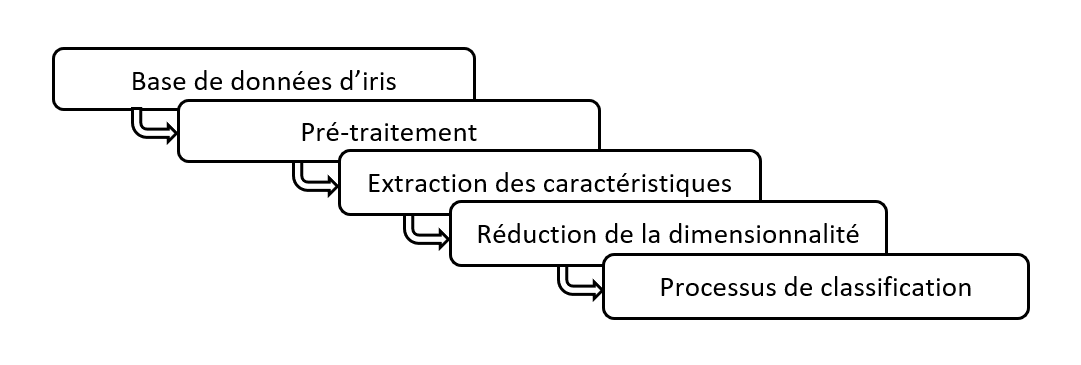
\includegraphics[width=0.9\linewidth]{schema}
        \captionof{figure}{Schéma du système.}
    \end{center}
    \vspace{1em}
    
    \section{Base de données}
    La base de donéees utilisée pour ce projet est « MMU iris dataset ». Elle est composée d’images d’oeil pour l’entraînement de modèles de système biométrique basé sur l’iris
de l’oeil. Cet ensemble de données se compose de 5 images de l’iris gauche et droit de
46 personnes.\cite{ref_2}

	\section{Pré-traitement}
	À cette étape, j'ai utilisé la méthode Hough Transform de scikit-image pour détecter l'iris dans les images. Ensuite, j'ai appliqué la technique « Warp Polar » de scikit-image pour transformer l'iris circulaire détecté en rectangle.\cite{ref_4} J'ai, par la suite, retiré la partie noire (la pupille) de l’image rectangulaire.
	
	
	\section{Extraction des caractéristiques}
	Pour l'extraction des caractéristiques, j'ai utilisé la méthode GLCM. Elle permet d'analyser les textures en calculant les répartitions des différents des niveaux de gris dans l'image en se basant sur les positions relatives des pixels. À partir de cette matrice, certaines caractéristiques de texture comme le contraste, l'énergie, l'homogénéité, etc. peuvent être identifiées.\cite{ref_5}
	
	\section{Réduction de la dimensionnalité}
	La réduction de la dimensionnalité est un processus qui consiste à réduire considérablement le nombre de caractéristiques pour faciliter le processus d’entraînement.\cite{ref_1} La méthode que j'ai utilisée est la PCA de scikit-learn.
	
	\section{Processus de classification}
    Pour la classification, j'ai utilisée la validation croisée et k-NN. La validation croisée consiste à séparer les données en, par exemple, 10 sous-groupes aléatoires pour l’entraînement. Ensuite, on entraîne et évalue les données 10 fois en choisissant 9 des sous-groupes pour l’entraînement et le dernier pour l’évaluation.\cite{ref_1} La méthode des k voisins les plus proches (k-NN) consiste à trouver les k échantillons dont l’entrée est la plus proche d’une nouvelle entrée.
    
    \vspace{1em}
    \begin{center}
        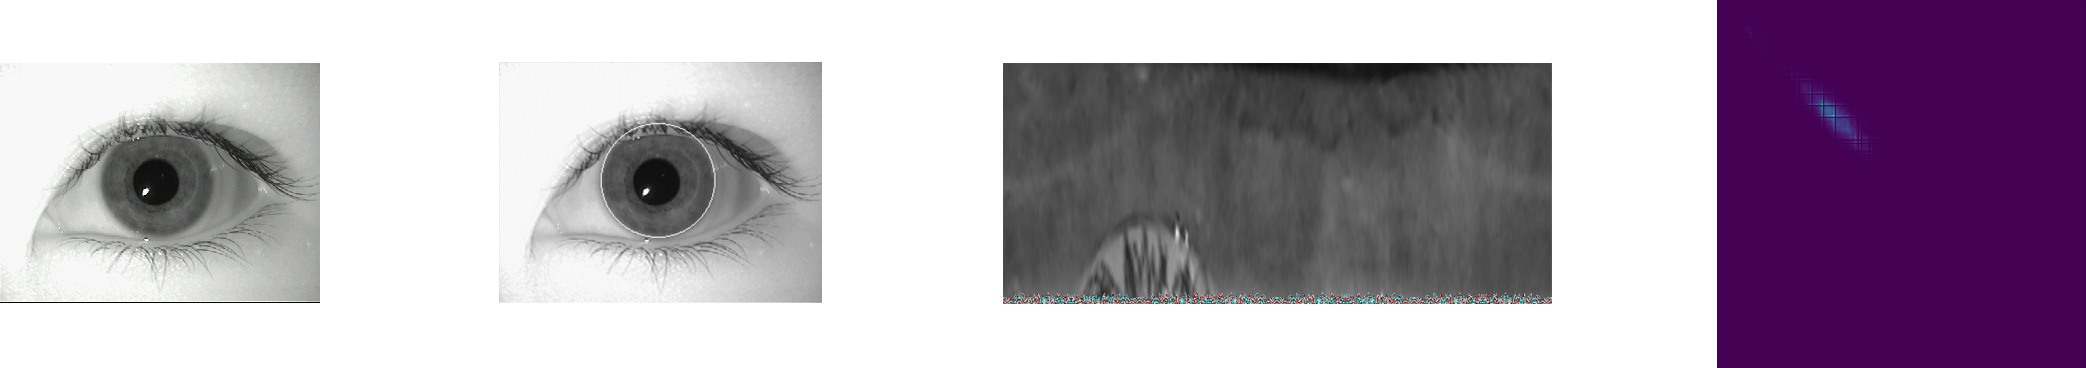
\includegraphics[width=0.9\linewidth]{processus}
        \captionof{figure}{Processus.}
    \end{center}
    \vspace{1em}
    
	}
}
 
    \column{0.32}
    \block{Méthodologie d'évaluation}{
 	{ \fontsize{40}{40}\selectfont 
 	
	\begin{itemize}
		\item[$\rightarrow$] La base de données de référence \href{https://www.kaggle.com/datasets/naureenmohammad/mmu-iris-dataset}{\textbf{MMU iris dataset}} a été téléchargée à partir de \textbf{Kaggle}.
		
		\item[$\rightarrow$] Caractéristiques biométriques pour $\mathbf{46}$ personnes, mais uniquement $\mathbf{10}$ sélectionnées aléatoirement ont été utilisées.
		
		\item[$\rightarrow$] Durant les évaluations, c'est la \textit{validation croisée} qui a été adoptée. Elle permet de générer $\mathbf{K = 10}$ parties \textit{stratifiés} afin d'éviter les biais.
	\end{itemize}	 	
	}
}

\block{Résultats préliminaires}{
 	{ \fontsize{40}{40}\selectfont 
 	
 	
 	    \begin{center}
			\captionof{table}{\selectfont Matrice de confusion pour \textbf{GLCM}-\textbf{PCA} et $k$-\textbf{NN}. }
			\vspace{0.3em}
			{ \fontsize{25}{25}\selectfont  	
				\begin{tabular}{l|c|c|c|c|c|c|c|c|c|c}
				Sujets & \textbf{005} & \textbf{010} & \textbf{013} & \textbf{022} & \textbf{027} & \textbf{030} & \textbf{032} & 						\textbf{035} & \textbf{038} & \textbf{040} \\ \hline
				\textbf{005} & \textbf{6} & 0 & 0 & 0 & 0 & 0 & 1 & 0 & 0 & 3 \\ \hline
				\textbf{010} & 0 & \textbf{9} & 0 & 1 & 0 & 0 & 0 & 0 & 0 & 0 \\ \hline
				\textbf{013} & 0 & 0 & \textbf{8} & 0 & 0 & 1 & 0 & 0 & 0 & 1 \\ \hline
				\textbf{022} & 0 & 1 & 0 & \textbf{8} & 1 & 0 & 0 & 0 & 0 & 0 \\ \hline
				\textbf{027} & 0 & 1 & 0 & 2 & \textbf{6} & 0 & 1 & 0 & 0 & 0 \\ \hline
				\textbf{030} & 2 & 0 & 1 & 0 & 0 & \textbf{4} & 1 & 0 & 0 & 2 \\ \hline
				\textbf{032} & 0 & 1 & 0 & 0 & 1 & 0 & \textbf{7} & 0 & 0 & 1 \\ \hline
				\textbf{035} & 0 & 1 & 0 & 0 & 1 & 1 & 0 & \textbf{7} & 0 & 0 \\ \hline
				\textbf{038} & 0 & 0 & 0 & 0 & 1 & 0 & 0 & 0 & \textbf{9} & 0 \\ \hline
				\textbf{040} & 0 & 1 & 1 & 0 & 0 & 1 & 0 & 0 & 0 & \textbf{7} \\ \hline
				\end{tabular}
			}
		\end{center}
    
    \begin{center}
		\captionof{table}{\selectfont Comparaison des deux méthodes.}
		\vspace{0.3em}
		{ \fontsize{30}{30}\selectfont 
    	\begin{tabular}{l|c}
        	Méthode 	& Taux de reconnaissance \\ \hline
            \textbf{GLCM}-\textbf{PCA} et $k$-\textbf{NN}   & $\mathbf{71\%}$ \\ \hline
            \textbf{GLCM} et $k$-\textbf{NN}     			& $22\%$ \\ \hline
    	\end{tabular}     		
    	}
    \end{center}
    \vspace{1em}
    
    }
}

\block{Conclusion}{
 	{ \fontsize{40}{40}\selectfont 
 	
	\begin{itemize}
		\item[$\checkmark$] Obtention de résultats intéressants avec la représentation \textbf{GLCM}-\textbf{PCA} qui est bien meilleure que la simple \textbf{GLCM} (+ \textit{caractéristiques}). 

		\item[$\checkmark$] Améliorer le processus de pré-traitement pour mieux détecter l'iris dans l'image et pour retirer le bruit comme les cils.
	\end{itemize}
    
    }
}
    
    \block{Références}{
    \fontsize{25}{25}\selectfont 
        \vspace{-3em}
	\bibliographystyle{plain}
	\renewcommand\refname{}
	\bibliography{fi3e_poster_refs}
    }
\end{columns}

\end{document}
